\documentclass[11pt]{article}
\usepackage [french]{babel}
\usepackage [T1]{fontenc}

\usepackage[linesnumbered, ruled, french, onelanguage]{algorithm2e}
\usepackage{adjustbox}%Permet de centrer les figures dans la largeur de la page même si les figures sont plus larges que \textwidth
\usepackage{amssymb}
\usepackage{amsmath}
\usepackage{adjustbox} % pour avoir adjustbox
\usepackage[toc,page,title,titletoc,header]{appendix}
\usepackage{expl3}%Pour la control sequence /ExlpSyntaxOn demandée par l'utilisation de subfiles apparemment...
\usepackage{gensymb}%pour pouvoir écrire le signe °
\usepackage{geometry}%Pour changer la largeur des marges du document notamment
\usepackage{graphicx}
\usepackage{hyperref}%pour les liens dans la bibliographie
\usepackage{listings}
\usepackage{placeins}%pour utiliser FloatBarrier afin que les figure respectent bien leur position dans le code
\usepackage{slashbox}%Case séparée en deux tout en haut à gauche des tableaux à double entrées
\usepackage{stmaryrd}%pour les crochets à double barres d'intervalles de nombre entiers
\usepackage{tikz}
\usepackage{xcolor}%/definecolor et /color
\usepackage{subfiles}

\usepackage{etoolbox}%pour /AtBeginEnvironment
\AtBeginEnvironment{appendices}{\renewcommand{\thesection}{\Alph {section}}}%Pour recommencer à compter les sections à 0 en rentrant dans l'annexe et pour compter avec des lettres et non des chiffres
\renewcommand{\appendixpagename}{\centering Annexes}%Pour centrer le titre de la partie annexe
\renewcommand{\appendixtocname}{Table des annexes} % Pour faire apparaître les annexes dans la table of contents
\setlength{\parskip}{2mm}%Pour mettre de l'espacement entre les paragraphes

\author{Tom CLABAULT - p2205453\\}
\title{
	\noindent\rule{\textwidth}{1pt}
	\textit{\textbf{TP Géométrie Algorithmique et maillage}}\\
	%{\small \textcolor{blue}{\href{https://github.com/TomClabault/M1-TP-TinyMesh}}}
	\noindent\rule{\textwidth}{1pt}
	\vskip 1cm
}
%\geometry{hmargin=3cm, vmargin=2cm}


\begin{document}
	
	\maketitle
	%\newgeometry{top=1in,bottom=1in,right=0.5in,left=1.5in}
	
	\section {Insertion de points}
	Afin de tester les algorithmes de Lawson et de Ruppert, quelques méthodes utilitaires d'insertion de points ont été nécessaires:

\begin{figure}[h!]
	\adjustbox{center}{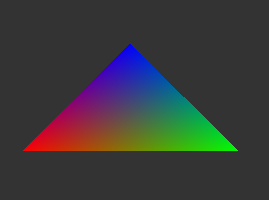
\includegraphics[width=0.4\textwidth]{Captures/Triangle.png}}
	
	\caption{Triangle d'origine}
\end{figure}
\FloatBarrier

\begin{figure}[h!]
	\adjustbox{center}{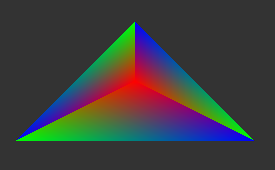
\includegraphics[width=0.4\textwidth]{Captures/InsertIn.png}}
	
	\caption{Insertion d'un point à l'intérieur d'un triangle: face split}
\end{figure}
\FloatBarrier

\begin{figure}[h!]
	\adjustbox{center}{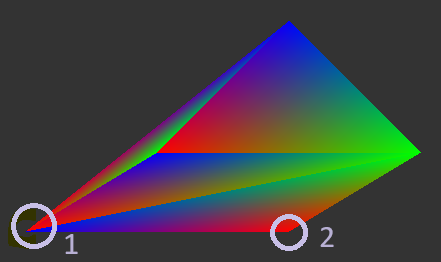
\includegraphics[width=0.4\textwidth]{Captures/InsertOut.png}}
	
	\caption{Simples insertions du point '1' puis du point '2' à l'extérieur du triangle d'origine}
	\label{InsertOut}
\end{figure}
\FloatBarrier
	\section {Algorithme de Lawson}
	L'algorithme de Lawson permet d'améliorer la qualité d'une triangulation en la rendant de Delaunay. L'algorithme procède itérativement:

\begin {itemize}
 \item {Étant donné une triangulation quelconque, on recherche les arêtes de la triangulation qui ne sont pas localement de Delaunay}
 \item {On place ces arêtes dans une file}
 \item {On flip ces arêtes une par une en prenant soin de vérifier que les arêtes voisines de celle qui a été flippée sont toujours localement de Delaunay (si elles ne le sont plus, elles sont elles aussi rajoutées à la file)}
\end {itemize}

\begin{figure}[h!]
	\adjustbox{center}{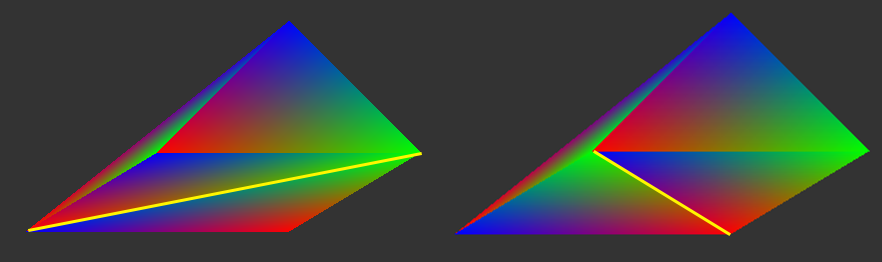
\includegraphics[width=0.8\textwidth]{Captures/BeforeAfterFlip.png}}
	
	\caption{Flip de l'arête jaune dans le triangle de gauche et résultat à droite}
\end{figure}
\FloatBarrier

L'algorithme de Lawson peut aussi être appliqué incrémentalement après chaque insertion de point dans la triangulation plutôt que sur le maillage entier:

\begin{figure}[h!]
	\adjustbox{center}{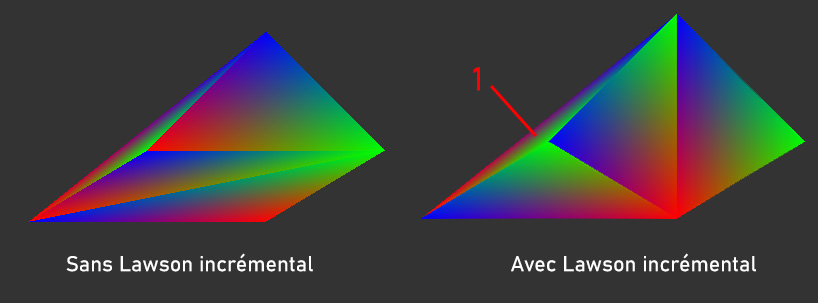
\includegraphics[width=0.8\textwidth]{Captures/InsertOutIncremental.jpg}}
	
	\caption{Insertion de deux points à l'extérieur du triangle de départ comme dans la \figurename \ref{InsertOut} avec et sans l'application de l'algorithme de Lawson incrémental à droite et à gauche respectivement. Le triangle 1 reste très plat à cause de son arête extérieure qui ne peut pas être flippée.}
\end{figure}
\FloatBarrier

\begin{figure}[h!]
	\adjustbox{center}{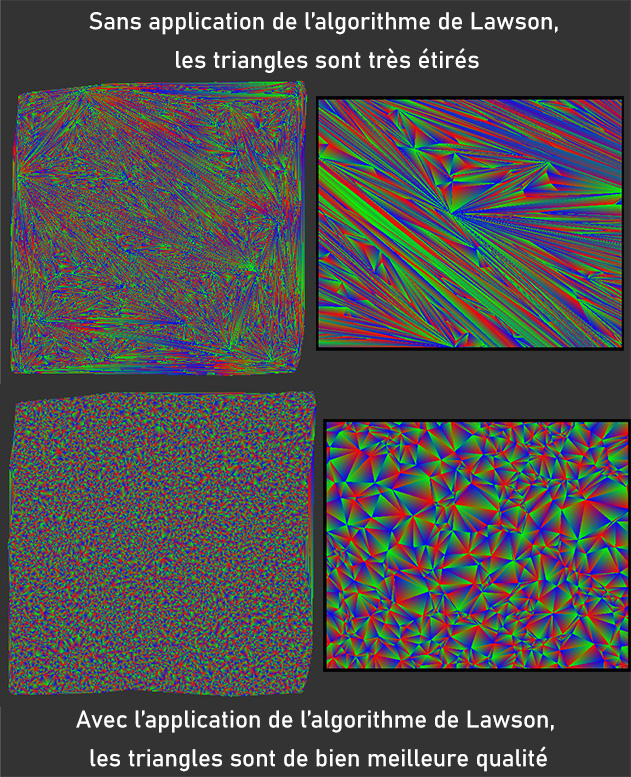
\includegraphics[width=0.8\textwidth]{Captures/TerrainNoVsIncremental.jpg}}
	
	\caption{Comparaison de la qualité des triangles pour l'insertion d'un large nombre de points avec et sans l'application de l'algorithme de Lawson (version incrémentale)}
\end{figure}
\FloatBarrier
	\section {Algorithme de Ruppert}
	L'algorithme de Ruppert permet de remplir (trianguler) une forme définie par un ensemble de segments (lui même constitué d'un ensemble de points). Les triangles ainsi formés respectent une certaine qualité définie par l'utilisateur: chaque triangle de la triangulation
finale devra avoir son plus petit angle supérieur à un seuil donné.

L'algorithme fonctionne en plusieurs étapes:
\begin {itemize}
	\item {On commence par créer une triangulation de Delaunay (Lawson incrémental) à partir des points donné en entrée à l'algorithme}
	\item {Une fois la triangulation obtenue, on vérifie que tous les segments de notre forme de départ font bien partie de notre triangulation.}
	\item {Pour chaque segment de la forme de départ qui ne fait pas partie de la triangulation, on insère un nouveau sommet au centre du segment, produisant deux nouveaux segments}
	\item {Si le segment ne fait toujours pas partie de la triangulation, on continue à découper récursivement les nouveaux segments}
	\item {Une fois tous les segments inclus dans la triangulation, on va insérer des nouveaux sommets au centre des cercles circonscrits aux triangles qui ne respectent par le seuil sur les angles donné. Le sommet est inséré au centre du triangle si et seulement si le sommet a insérer ne tombe pas dans le cercle diamétral d'un des segments de contrainte.}
	\item {Le résultat est une triangulation de Delaunay avec une garantie de qualité (seuil sur les angle des triangles) qui contient tous les segments de la forme de départ.}
\end {itemize}

\begin{figure}[h!]
	\adjustbox{center}{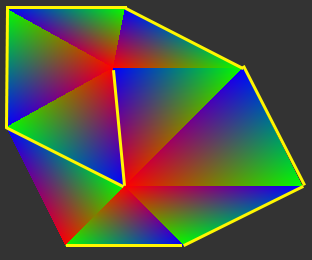
\includegraphics[width=0.6\textwidth]{Captures/RuppertSegments.png}}
	
	\caption{Les segments de contraintes sont représentés en jaune. L'algorithme de Ruppert permet de trianguler la forme.}
\end{figure}
\FloatBarrier

\end{document}
